\section{Research orientation for MMALS}

\subsection{Why synthetic-data collapse maps naturally to MMALS}

MMALS does not only process external datasets. It also produces internal artefacts:
\[
\text{context}
\rightarrow
\text{host activations}
\rightarrow
\text{route}
\rightarrow
\text{memory trace}
\rightarrow
\text{future routing evidence}.
\]
If these artefacts are replayed, summarized, or used as pseudo-labels for later versions, MMALS becomes a recursive data-generation system. The analogue of a token distribution is a distribution over functional regimes, hosts, routes, memories, and collaborative trajectories.

Let $r\in\mathcal R$ denote a route and let
\[
p_g(r\mid x,m,z)
\]
be the routing distribution at generation or learning cycle $g$. A self-reinforcing loop can occur:
\[
p_g(r)
\rightarrow
D_g^{\mathrm{trace}}
\rightarrow
\text{router update}
\rightarrow
p_{g+1}(r).
\]
A route that is slightly more frequent receives more replay, more gradient, and more memory support. This can increase its probability even when its original advantage was accidental.

\subsection{Functional model collapse}

We define \emph{functional model collapse} as a reduction in the effective set of accessible, causally useful behaviours while average performance or route stability may remain high.

A practical definition requires four elements:

\begin{enumerate}[leftmargin=*]
  \item a target distribution of functional regimes $P_{\mathrm{target}}$;
  \item a set of accessible routes $\mathcal R_g$;
  \item a causal utility test $U(r)$;
  \item a comparison across learning cycles or generations.
\end{enumerate}

The effective functional support can be written conceptually as
\[
K_{\mathrm{eff}}(g)
=
\sum_{r\in\mathcal R}
\ind\left[
\Prob_g(r)>\epsilon_p,
\Delta Q_r^{\mathrm{causal}}>\epsilon_q
\right].
\]
A collapse occurs when $K_{\mathrm{eff}}$ decreases materially and the missing routes correspond to real target regimes.

\begin{figure}[H]
\centering
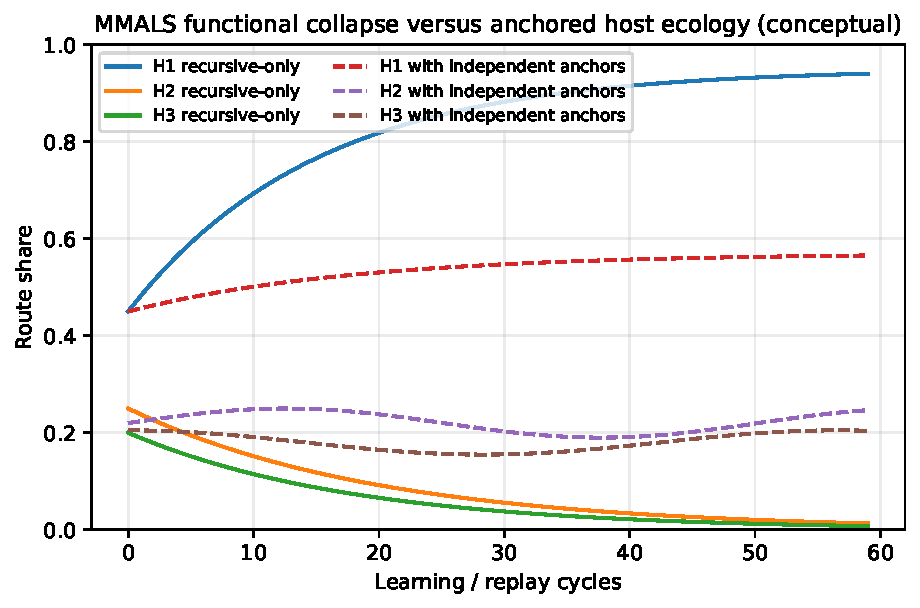
\includegraphics[width=0.90\textwidth]{figures/mmals_host_ecology.pdf}
\caption{Conceptual host ecology under recursive-only reinforcement and under continued independent anchoring. The figure is illustrative, not an empirical MMALS result.}
\label{fig:mmals-ecology}
\end{figure}

\subsection{The two collapse mechanisms in MMALS}

The two mechanisms highlighted in synthetic-data research have direct analogues.

\paragraph{Finite sampling of routes.} A useful route is rare. It is absent from replay batches, audit memory, or synthetic traces. Its hosts receive no reinforcement. Eventually the route becomes practically inaccessible.

\paragraph{Function-approximation error.} The shared latent space, energy function, or router cannot preserve all relevant regimes. Several distinct routes are smoothed into a single dominant solution.

A third MMALS-specific mechanism should be added:

\paragraph{Objective-induced collapse.} A fixed or dominant objective---for example immediate accuracy---systematically suppresses routes useful for retention, cost, stability, or future recomposition. This is especially relevant to TPUT and goal-conditioned control.

\subsection{Softmax, temperature, and route tails}

Suppose route scores are energies $E_r$ and
\[
p(r\mid x)
=\frac{\exp(-E_r/\tau)}{\sum_{r'}\exp(-E_{r'}/\tau)}.
\]
A lower temperature concentrates routing. This can be appropriate when one route is clearly superior. It is dangerous when uncertainty remains or when the concentration is reused as training truth.

The key distinction is:
\[
\text{local concentration at inference}
\neq
\text{global deletion from learning support}.
\]
MMALS should be able to use one host for a simple input while retaining other routes in the global ecology.

Hard top-$k$ or top-$p$ routing can create an exact analogue of chopped tails: routes outside the selected set receive no activity and potentially no learning signal. A softmax router with only a few parameters may therefore outperform a more elaborate hard selector if it preserves uncertainty and avoids premature support loss.

\subsection{Natural adaptability without controller proliferation}

The architectural objective established in the preceding MMALS work is not to accumulate separate boxes for routing, tail preservation, synthetic-data control, collapse prevention, novelty detection, and memory governance. Instead, a small number of local laws should generate the desired global behaviour.

Let the MMALS state be
\[
S_t=(z_t,h_t,m_t,a_t,W_t),
\]
where $z_t$ is latent context, $h_t$ host states, $m_t$ memory, $a_t$ activity allocation, and $W_t$ interaction structure. A generic dynamics is
\[
S_{t+1}
=S_t-\eta\nabla_S\mathcal E(S_t;x,g)
+\mathcal P(S_t)+\xi_t.
\]
The energy should combine task residual, cost, instability, forgetting, and unsupported redundancy:
\[
\mathcal E
=
\mathcal E_{\mathrm{task}}
+\lambda_C C
+\lambda_S \mathcal E_{\mathrm{stability}}
+\lambda_F \mathcal E_{\mathrm{forgetting}}
+\lambda_R \mathcal E_{\mathrm{redundancy}}.
\]
Synthetic lineage and verification should not necessarily become a central controller. They can become state variables that modulate local consolidation.

\subsection{Lineage-aware memory consolidation}

A memory trace can be represented as
\[
m_j=(z_j,r_j,y_j,s_j,g_j,v_j,f_j,c_j),
\]
where:

\begin{itemize}[leftmargin=*]
  \item $z_j$ is context;
  \item $r_j$ is route;
  \item $y_j$ is result;
  \item $s_j$ is source class;
  \item $g_j$ is synthetic generation depth;
  \item $v_j$ is verification strength;
  \item $f_j$ is freshness;
  \item $c_j$ is causal contribution evidence.
\end{itemize}

A conceptual consolidation law is
\[
\Delta M_j
\propto
\underbrace{\Delta Q_j^{\mathrm{verified}}}_{\text{functional gain}}
\times
\underbrace{N_j}_{\text{novelty}}
\times
\underbrace{I_j}_{\text{independence}}
\times
\underbrace{F_j}_{\text{freshness}}
\times
\underbrace{e^{-\lambda g_j}}_{\text{lineage discount}}.
\]
This expression is not proposed as a final formula. It identifies variables that should be represented explicitly and then simplified by experiment.

\begin{mmalsnote}
A trace should not become true because it is frequent. It should become influential because it remains useful under an independent residual, a causal intervention, or a verified external objective.
\end{mmalsnote}

\subsection{Reconstructive and synthetic memory}

The lecture sharpens the distinction between the two planned MMALS memory modes.

\paragraph{Reconstructive audit memory.} Stores the route, intermediate states, sources, and verification metadata required to replay or audit a decision. Its value is traceability, not compression.

\paragraph{Synthetic or compiled functional memory.} Compresses repeated successful experiences into reusable structure. Its value is low-cost transfer and abstraction.

The collapse risk is asymmetric. Reconstructive memory can become an enormous exact-match table. Synthetic memory can over-compress and remove rare distinctions. The two should constrain each other:
\[
\text{audit traces}
\leftrightarrow
\text{compiled functions}.
\]
A compiled function should remain linked to representative traces, including counterexamples and boundary cases.

\subsection{Host specialization and tail preservation}

A rare host is not automatically valuable. A dominant host is not automatically pathological. Host value should be claim-relative:
\[
V(H_i)
=\sum_r P(r)\,L(r)\,\Delta Q_{i,r}^{\mathrm{causal}}-C(H_i),
\]
where $L(r)$ is regime criticality and $C(H_i)$ the cost of maintaining or activating the host.

This leads to a better tail metric than route entropy alone. Define functional tail coverage
\[
\mathrm{FTC}
=\sum_{r\in\mathcal R_{\mathrm{tail}}}
P_{\mathrm{eval}}(r)
\ind[\Delta Q_r^{\mathrm{causal}}>0].
\]
FTC measures the probability mass of rare regimes for which MMALS retains a causally useful route.

The existing host-specialization programme should therefore combine:

\begin{itemize}[leftmargin=*]
  \item route entropy and dominance;
  \item host contribution gain;
  \item ablation impact;
  \item route swaps and candidate permutations;
  \item representation separation;
  \item route-function stability;
  \item cross-seed reproducibility;
  \item functional tail coverage;
  \item synthetic lineage depth.
\end{itemize}

\subsection{Dynamic compute as a scaling law}

MMALS should distinguish installed capacity and effective capacity:
\[
d_{\mathrm{installed}}
\quad\text{versus}\quad
 d_{\mathrm{eff}}(x)=\sum_i a_i(x)d_i.
\]
The desired property is
\[
d_{\mathrm{eff}}(x_{\mathrm{simple}})
\ll
d_{\mathrm{eff}}(x_{\mathrm{complex}}),
\]
without changing the global architecture.

A useful objective is
\[
\min_{r,a,T_{\mathrm{iter}}}
\left[
\mathcal L(x;r,a)
+\lambda_C C(r,a,T_{\mathrm{iter}})
+\lambda_F F(r)
\right].
\]
The system should spend additional computation only when it produces a measurable reduction in residual or future risk. Importantly, a difficult but invalid or corrupted input should not trigger unlimited computation. One stable state must be abstention.

\subsection{Choice of Llama or Mistral backbones}

MMALS should not be defined by a single LLM family. The scientific design should use a stable host interface:
\[
\texttt{encode},\quad
\texttt{forward},\quad
\texttt{adapt},\quad
\texttt{uncertainty},\quad
\texttt{export\_trace}.
\]

For causal host-specialization experiments, the first stage should use the same dense base backbone for all hosts, with equal parameter budgets and controlled adapters. This prevents backbone heterogeneity from masquerading as emergent specialization. A second stage should replicate the results with a different model family. A third stage may introduce heterogeneous hosts.

The selection principle is therefore:

\begin{enumerate}[leftmargin=*]
  \item choose a dense base model that fits the available hardware;
  \item avoid internal MoE routing in the first causal study;
  \item freeze exact model, tokenizer, quantization and adapter versions;
  \item use one family as the primary experiment and another as replication;
  \item compare cross-tokenizer metrics using bits-per-byte or relative deltas rather than raw perplexity alone.
\end{enumerate}

This is more durable than declaring MMALS a ``Llama architecture'' or a ``Mistral architecture.'' The backbone is a host; MMALS is the organisation of hosts.

\subsection{MMALS hypotheses generated by the lecture}

\begin{description}[leftmargin=3.2cm,style=nextline]
  \item[H1: Recursive route collapse.] Training primarily on self-generated routes reduces functional tail coverage across generations.
  \item[H2: Real-anchor recovery.] A sufficiently diverse stream of independently verified experiences restores lost route support after a delayed transition.
  \item[H3: Verification bootstrap.] Over-generating route candidates and verifying them can train a later MMALS version beyond the initial router's top-1 performance.
  \item[H4: Dynamic temperature.] State-dependent route temperature improves the cost--accuracy trade-off relative to fixed hard routing without increasing structural complexity.
  \item[H5: Dual-memory protection.] Linking compiled memories to reconstructive counterexamples reduces recursive memory collapse.
  \item[H6: Geometry-sensitive support.] A manifold-aware latent state preserves distinct functional regimes that are smoothed together in a Euclidean representation.
\end{description}

\subsection{What would count as a strong MMALS result?}

A strong result would not be ``MMALS retains high route entropy.'' It would show:

\begin{enumerate}[leftmargin=*]
  \item simple cases use short, inexpensive routes;
  \item hard cases recruit additional hosts only when they improve a verified residual;
  \item rare useful routes survive recursive replay;
  \item lost routes can be recovered by diverse real anchors;
  \item candidate verification produces a student that outperforms the teacher's top-1 routing;
  \item these effects replicate across seeds, datasets, and at least two backbone families;
  \item ablations demonstrate that memory, geometry, and collaboration are causally necessary for the claimed gains.
\end{enumerate}
